%% BioMed_Central_Tex_Template_v1.06
%%                                      %
%  bmc_article.tex            ver: 1.06 %
%                                       %

% !TEX TS-program = xelatex
\documentclass{bmcart}


\usepackage[utf8]{inputenc} 
%\usepackage[margin=2cm]{geometry}
%\usepackage{colortbl}
\usepackage{comment}
%\usepackage{caption}
%\usepackage{subcaption}
\usepackage{mathptmx}
\usepackage{nicefrac}
%\usepackage{authblk}
\usepackage{array}

\usepackage{times}
\usepackage{lineno}
\usepackage{cite}
%\usepackage[round]{natbib}
%\makeatletter
%\renewcommand{\@biblabel}[1]{#1.}
%\makeatother

\usepackage{graphicx}
\usepackage{amsmath}
\usepackage{xcolor}

\def\includegraphic{}
\def\includegraphics{}

\startlocaldefs
%\usepackage{url}
%\urlstyle{same}

\graphicspath{{figures/}{./}}

%\usepackage[small,compact]{titlesec}
%\titleformat{\section} {\vspace{24pt}\bf\sffamily\MakeUppercase}{\thesection} {0pt} {}
%\titleformat{\section} {\vspace{12pt}\bf\large}{\thesection}{0pt}{}
%\titleformat{\subsection} {\vspace{6pt}\bf}{\thesubsection} {0pt} {\vspace{-2pt}}
%\titleformat{\subsubsection} [runin] {\bf}{\thesubsubsection} {12pt} {}

\newcolumntype{+}{>{\global\let\currentrowstyle\relax}}
\newcolumntype{^}{>{\currentrowstyle}}
\definecolor{badpatcol}{HTML}{FF6666}
\newcommand{\badpat}{\gdef\currentrowstyle{\bfseries}\bfseries\ignorespaces }

\newcounter{subfigure}[figure]
\newcounter{subfiguresmall}[figure]
\newcommand{\sublabel}[1]{\refstepcounter{subfigure}\label{#1}\refstepcounter{subfiguresmall}\label{#1small}}
\renewcommand{\thesubfigure}{\thefigure \alph{subfigure}}
\renewcommand{\thesubfiguresmall}{\alph{subfiguresmall}}
\newcommand{\subref}[1]{\ref{#1small}}

\endlocaldefs

%\captionsetup[subfigure]{width=0.9\textwidth}
 
%\newcommand{\tabletitle}[1]{\caption*{\bfseries #1}\vspace{-10pt}}
%\newcommand{\figtitle}[1]{\caption*{\Large \bfseries #1}}
%\newcommand{\figtitlel}[1]{\subcaption[\large \bfseries]{#1}}

\begin{document}

%\pagewiselinenumbers

\begin{frontmatter}

\begin{fmbox}

\dochead{}

\title{Blind dating: a phylogenetic approach to determining the ages of HIV-1 reservoir sequences within host}

\author[addressref={1,2},email={brj1@sfu.ca}]{Bradley R. Jones} % brj1@sfu.ca
\author[addressref={1,2},email={jjh13@sfu.ca}]{Joshua Horacsek} % jjh13@sfu.ca
\author[addressref={2,3},email={jjoy@cfenet.ubc.ca}]{Jeffrey B. Joy} % jjoy@cfenet.ubc.ca
\author[addressref={1,2},email={zbrumme@sfu.ca}]{Zabrina L. Brumme} % zbrumme@sfu.ca
\author[addressref={2,3},email={apoon@cfenet.ubc.ca},corref={3}]{Art F.Y. Poon} % apoon@cfenet.ubc.ca
\address[id=1]{\orgname{Faculty of Health Sciences, Simon Fraser University} \city{Burnaby} \cny{Canada}}
\address[id=2]{\orgname{BC Centre for Excellence in HIV/AIDS} \city{Vancouver} \cny{Canada}}
\address[id=3]{\orgname{Department of Medicine, University of British Columbia} \street{2775 Laurel Street} \city{Vancouver} \postcode{V5Z 1M9} \cny{Canada}}
%\affil[*]{Corresponding author}

brj1@sfu.ca, jjh13@sfu.ca, jjoy@cfenet.ubc.ca, zbrumme@sfu.ca, apoon@cfenet.ubc.ca
 
\printaddresses

%%% 1 Simon Fraser University
%%% 2 BC Centre for Excellence in HIV/AIDS
%%% 3 University of British Columbia
%\baselineskip 30pt


\begin{artnotes}
\end{artnotes}

%\maketitle
\end{fmbox}

\begin{abstractbox}
\begin{abstract}
\paragraph{Background:}
The ability of HIV to persist within latent cellular reservoirs represents a major barrier to
%developing an effective
cure.
The timing of establishment of individual viral reservoirs over the course of an infection may influence their susceptibility to elimination by immune-mediated or therapeutic approaches.
However, methods to accurately estimate the age of reservoir sequences remain scarce.
We propose a simple method to date suspected reservoir sequences using phylogenetically informed regression.
 
% Possibly fix these subsections
\paragraph{Results:}
%Simulated sequence data were generated.
%A total of 410 HIV RNA sequences sampled longitudinally from 9 untreated HIV-infected individuals with estimated dates of infection and a total of 2816 HIV DNA and RNA sequences from 20 individuals were obtained from the Los Alamos National Laboratory HIV Sequence Database.
%The simulated and HIV RNA data were used for method validation.
Our method is as follows: Taking aligned HIV sequences from a single individual sampled over multiple time points, we reconstruct a maximum-likelihood phylogeny.
The location of the root in the phylogeny is determined using root-to-tip regression.
%The phylogeny is rooted by determining the location of the root using root-to-tip regression.
Finally, the root-to-tip distances of possibly latent sequences are mapped to the optimal regression line to estimate reservoir establishment dates.
%Finally, the presence of latent lineages within () was detected using a nonparametric binary test.
To validate our method, we simulated HIV sequence evolution under a standard model and reconstructed phylogenies from these data by maximum likelihood.
Latency was simulated by shortening the branch lengths of up to 50\% of the tips in the tree.
We employed this same approach to validate the method on HIV RNA sequences, which provided a more realistic assessment of sources of error than direct simulation.
%We synthesized latent lineages by censoring the sample dates for random selections of up to 50\% of sequences in the simulated and HIV RNA datasets.
When this method was applied to HIV DNA sequences in phylogenies containing dated HIV RNA sequences, we observed that the predicted dates significantly preceded dates of sampling, which was consistent with latency.

\paragraph{Conclusion:}
Our results provide evidence that the date that a lineage of HIV entered a latent state can be reconstructed from phylogenetic analysis of HIV RNA sequence variation from the same patient.
These dates can provide important insights into the dynamics of HIV reservoirs within hosts.


\paragraph{Keywords:} 
HIV, Latency, Cellular Reservoirs, Phylogenetics, Linear Regression
\end{abstract}
\end{abstractbox}
\end{frontmatter}

\baselineskip 30pt

\section * {Background} \label{sec:intro}

HIV-1, like all retroviruses, integrates its genome into the chromosome of the infected host cell during the viral life cycle.
Though the vast majority of infected cells die as a result of viral cytopathic effects or immune-mediated elimination, a small minority (broadly estimated as one in every million resting CD4+ T-cells \cite{Chun97,Finzi97}) harbour integrated HIV DNA in a state of near or complete transcriptional quiescence over long time periods \cite{Archin14,Pace11,Richman09}.
Termed latent HIV-1 reservoirs, such cells represent a major obstacle in curing HIV-1 infection as they can persist for years.
In the presence of suppressive antiretroviral therapy, for instance, these reservoirs can be re-activated at any point to produce infectious virus, thereby reseeding infection \cite{Richman09,Durand12,Joos08,Katlama13,Pomerantz03,Shen08}. 

Establishment of individual viral reservoirs within a given host  begins within hours or days following infection and continues thereafter \cite{Whitney14,Leford14}.
As within-host HIV-1 populations rapidly accumulate genetic diversity over the course of an infection \cite{Alizon13,Rambaut04,Shankarappa99}, latent viral genomes present during untreated chronic infection should be heterogeneous in terms of age and genetics, ranging from those archived soon after infection (that resemble ancestral viruses within the host) to those that have integrated relatively recently into cellular reservoirs (that resemble contemporary plasma strains).
The chronology of establishment and genetic distribution of latent HIV-1 lineages within a given host is may be relevant to the development of strategies to eliminate them, as these properties could influence their susceptibility to reactivation and/or immune-mediated clearance.
For example, while the `oldest' reservoirs within a given individual may be the most inherently refractory to reactivation with latency reversing agents, `younger' reservoirs may be largely refractory to subsequent immune-mediated elimination due to an accumulated burden of immune escape mutations \cite{Deng15}.
However, within-host dynamics of HIV-1 reservoir establishment remain incompletely characterized.
Previous studies have developed techniques to detect latent lineages by reduced rates of viral evolution \cite{Immonen14} and modelled the population dynamics of different classes of the virus within a given host \cite{Althaus14}.
However, there has been limited research on estimating when known or suspected latent viral lineages originally became integrated into their respective host cell genomes, or qualitatively assessing the age distributions of latent HIV-1 lineages within a given host.  

We here describe a novel phylogenetic method to `date' individual viral reservoir sequences within a host.
The method utilizes longitudinal plasma HIV RNA sequences sampled over an individual's infection to calibrate a host-specific HIV evolutionary rate from which the ages of known or suspected reservoir sequences are then inferred. The premise is as follows.
Because HIV-1 sequences within a given infected host rapidly accumulate genetic diversity due to HIV-1's high mutation rate and short generation time \cite{Alizon13,Rambaut04,Shankarappa99}, it is possible to reconstruct a phylogenetic tree that represents the ancestor-descendant relationships between HIV-1 sequences sampled longitudinally from within that host.
A phylogeny that is reconstructed by parametrizing a model of molecular evolution solely on the basis of sequence homology (\emph{e.g.}, by maximum likelihood estimation \cite{Felsenstein81}) has branch lengths in units of expected numbers of substitutions, in which the passage of time is confounded with the rate of evolution.
In other words, a tree that stretches far back in time with a slow rate of evolution will explain a given set of sequences just as effectively as a shallow tree with rapid evolution.
When sampling dates are known however, the corresponding tips of the phylogeny can be fixed at these time points, allowing the rate of evolution to be estimated directly \cite{Rodrigo99}.
Knowledge of sampling dates thus enables one to rescale a phylogeny in chronological time, which is especially useful for within-host HIV-1 populations in which substantial genetic differences can accumulate in weeks or months \cite{Williamson03}.
Moreover, among the actively replicating HIV lineages within a host, the rate of molecular evolution is fairly consistent over time \cite{Korber00,Kuhner95,Leitner99,Park16}.
Consequently, the divergence of descendant lineages from the transmitted/founder virus can be approximated by a `strict' molecular clock model in which a consistent rate of evolution is sustained, at least over the initial years, of an individual's infection course \cite{Keele08}. 

Upon integration of a given HIV-1 sequence into a host cell genome, evolution of that lineage effectively ceases until a new round of virus replication ensues.
Latent HIV-1 sequences will therefore display a characteristic discordance between their sampling date and their apparent (younger) age based on sequence divergence from other within-host lineages (where the latter age reflects the date on which that HIV-1 sequence originally integrated into the host cell genome; see Figure \ref{fig:latenttree}).
Our method is therefore based on the premise that we can use within-host phylogenetic analysis to estimate the original integration dates of known or suspected latent HIV-1 sequences.
Assuming that within-host HIV-1 evolution can be adequately modelled by a strict molecular clock such that the expected number of substitutions per site increases linearly with time \cite{Ho14}, we construct a phylogeny relating sequences derived from plasma HIV-1 RNA sequences sampled longitudinally from within a given host. We then parametrize a strict molecular clock by fitting a linear model to the known HIV RNA collection dates and the path lengths from the corresponding tips of the phylogeny to the inferred tree root (which represents the earliest point in time in the phylogeny).
Next, we use the linear model to reconstruct tip dates of HIV-1 sequences for which sampling dates were masked. 
We employed simulated and real longitudinal HIV sequence data to evaluate model accuracy, and finally applied the model to estimate the distribution of integration dates of viral lineages sampled as cellular HIV DNA in real longitudinal data sets.

%%%%%%%%%%%%%%%%%%%%%%%% METHODS %%%%%%%%%%%%%%%%%%%%%%%%%%

\section * {Methods} \label{sec:methods}

\subsection * {Data sets}
For our experiments, we compiled five data sets of real and synthetic longitudinal HIV sequences.
Three of the data sets comprised of simulated data --- two of which had viral latency incorporated into their models.
The other two data sets were comprised of real HIV-1 \emph{env} sequences --- one data set contained sequences only from HIV RNA extracted from plasma and the other contained both plasma HIV RNA and HIV DNA extracted from PBMC.

\subsubsection * {Simulated data.} \label{subsec:simdata}

%%% 1. simulate trees with strict clock - baseline
%%% 2. directly manipulate plasma trees
%%% 3. simulate sequence evolution on trees - additional error

To characterize sources of error in reconstructing dates on tips of a phylogeny, we generated phylogenetic trees by direct simulation. % and from the plasma data sets.
First, we generated phylogenies with 100 tips each under a birth-death model with serial sampling using the \emph{sim.bdsky.stt} function in the \textit{R} package \textit{TreeSim} \cite{Boskova14}.
Birth-death models have been applied to studying speciation processes \cite{Nee:2006} and infectious disease epidemics \cite{Stradler13}, but have only recently been used to model the proliferation of virus lineages in cell populations \cite{Hartfield:2015}.
%% This paragraph needs to be rewritten
The birth-death model was parametrized by fitting this model to samples from the {\em plasma} dataset.
%% we may need to provide some justification for using BD
%To assess the sensitivity of our method, we first simulated HIV sequence data sets without viral latency.
We used BEAST version 2.3.2 \cite{BEAST2} to estimate the posterior distribution defined by the serial model with a Bayesian skyline \cite{Stadler13}, a strict molecular clock, and the HKY85 \cite{HKY85} model of nucleotide substitution.
%Using this approach, we generated samples of trees for each sequence alignment in the plasma dataset.
%From these simulations, we evaluated the accuracy of predicting sample collection times from a strict molecular clock model that was fit to a training subset of these data.
The lineage birth rate, death rate and sampling probability were estimated to be: $\lambda = 5.12 \times 10^{-2}$ day$^{-1}$, $\delta = 5.01 \times 10^{-2}$ day$^{-1}$, $s = 5.24 \times 10^{-3}$ respectively.
We used the \textit{R} package, \emph{NELSI} \cite{NELSI}, to assign rates of evolution to these trees by drawing values from a Gaussian distribution with a mean rate $\mu = \ 1.96\times 10^{-4}$ substitutions per generation and standard deviation $\sigma = \ 1.42\times 10^{-5}$. %; Figure \ref{fig:seedtree} for an example).

To model uncertainty in phylogenetic reconstruction from sequence variation, we simulated sequence evolution along each birth-death tree with INDELible version 1.03 \cite{Indelible09} under an HKY85 \cite{HKY85} model of nucleotide substitution.
Parameters for the substitution model were set to empirical estimates derived from previously published HIV within-host data sets \cite{McCloskey14}. 
Specifically, the stationary distribution was set to 0.42, 0.15, 0.15, 0.28 for the nucleotides A, C, G and T, respectively, and the transition bias parameter was set to 8.5.
Using this approach, we generated a total of 50 replicate subjects without viral latency.
We will call the set of these subjects the \emph{simulated (no latency)} data set.

%A phylogeny was reconstructed from the simulated sequence alignments using the approximate maximum likelihood heuristic implemented in FastTree2.
%Similar results were obtained with trees reconstructed using RAxML \cite{Raxml14}, which is expected to be more accurate, but can consume orders of magnitude more computational time.

To simulate phylogenies with latent viral lineages, we employed an approach similar to \cite{Immonen14}, but with the simplifying assumptions that any sampled virus lineage could undergo no more than one latent period, and that once a lineage entered a latent state, it remained latent until becoming sampled.
To do this, we selected 50 tips uniformly at random from each `latency-free' phylogeny, then shortened their expected number of substitutions and their branch time (the time between the tip, and the tip's parent).
To this end, we applied two different methods.
The first method was an extreme case used as a baseline where we shortened each chosen tip's branch time by either 100 days or by a factor of $0.99$ of the branch time if the branch time was less than 100 days.
The second method was intended to be more realistic and is as follows. For each chosen tip:
\begin{enumerate}
\item Draw a random period for latency, $L$, from an exponential distribution with rate, $l$.
\item Draw a random waiting time to integration, $I$, from a restricted exponential distribution with rate, $i$, and bounds $\max\{S-L, 0\}$ and $S$, where $S$ is the branch time of the tip.
\item Shorten the branch time to equal $I$.
%\item Scale the expected number of substitutions.
\end{enumerate}
See Figure \ref{fig:latencymodel} for an illustration of this model.

We derived the parameters, $l$ and $i$, from results found in the literature.
We computed $l$ from the mean half life of latently infected CD4$^+$ T-cells ($3.6$ years) estimated in \cite{Crooks15}.
Using this estimate, we calculated $l = 5.3 \times 10^{-4}$ day$^{-1}$.
Similarly, we parametrized $i$ from the frequency of latently infected CD4$^+$ T-cells found by \cite{Ho13} ($i = 3. \times 10^{-4}$ day$^{-1}$).
%For the second set we calculated $l = 2.8 \times 10^{-4}$ day$^{-1}$ and $i = 1.5 \times 10^{-4}$ day$^{-1}$ based on the model of \cite{Kim06}.
%See Supplementary Materials S1 for details.
%% For supplementary
%We took $u$ to equal their $a_0 = c\frac{V_0}{NL_0}-(1-f)(1-\epsilon)kT_0\frac{V_0}{L_0}$ with $c = \delta$, $N = \lambda$,  $\frac{V_0}{L_0} = f$, $\epsilon = 0$, $k = \lambda$, $T_0 = 1$ and $f = 0.003$.
%This gives $u = 0.00028$.
%We took $l = f(1-\epsilon_{RT})k$ with $\epsilon_{RT} = 0$ and $f$ and $k$ as above.
%Using this approach, we get $l = 0.00015$.
Next, we recorded both the simulated waiting time to latency and the simulated collection time and generated sequences along these latent seed trees with INDELible using the same parameters as above.
The set of simulated subjects created from each of these methods comprise the \emph{simulated (extreme)} and \emph{simulated (latency)} data sets respectively.
For these data, we generated an additional 100 subjects with 100 sequences each, bringing the total amount of simulated data to 150 subjects and 20,000 sequences.


\subsubsection * {Data collection.} \label{subsec:dcollection} % Collection of real data
We collected two distinct sets of real data for our experiments. 
The first we refer to as the {\em plasma} data set, which comprised of sequences derived from viral RNA from longitudinal plasma samples \cite{McCloskey14}. 
From these data, we selected treatment naive individuals with two or more clonal or single-genome sequences available at each time point, and with a known time-line relative to one of several reference points: HIV infection, seroconversion or presentation of symptomatic seroconversion illness. 
The baseline samples were collected within 186 days of this reference point, and at least one of the subsequent `follow-up' time points occurred a minimum of 6 months after baseline.
Individuals who had been classified as `superinfected' were also excluded \cite{McCloskey14}.
After applying these criteria, we retained 410 HIV RNA sequences from 9 individuals for phylogenetic analysis.
The purpose of the plasma data set was to provide representative samples of within-host HIV diversity for evaluating and calibrating the model.

The second data set, referred to as the {\em mixed} data set, contained sequences from studies in which both plasma HIV RNA and cellular HIV DNA had been collected from the same individual.
We used the advanced search interface of the Los Alamos National Laboratory (LANL) HIV Sequence Database \cite{LosAlamos} to identify published data sets representing individuals with both HIV RNA and cellular DNA sequences.
%% what do you mean by "well-characterized"?
From these results, we manually selected 20 individuals that had well-characterized partial {\em env} sequences and plasma samples from at least 2 RNA time points and 3 DNA time points. 
%We also required that at least 1 RNA time point fell between 2 DNA time points in each individual
There were no other selection criteria on the time between sample collection dates. 
A total of 1,017 partial {\em env} sequences from blood plasma, and 1,799 partial {\em env} sequences from PBMC cells were used in our analysis. 
We utilized samples from treatment naive individuals from \cite{Shankarappa99, Novitsky09} and samples from individuals that had been intermittently treated via HAART from \cite{Llewellyn06,Fischer04}. 
See Table \ref{tab:patients} for details on the patients from these data sets.

\begin{table*}
\def\arraystretch{1.3}%
\begin{center}
\begin{tabular}{llrrrrrrr} 

Reference & Patient ID & \multicolumn{3}{c}{Sequences} & \multicolumn{3}{c}{Time points} \\
 &  & Plasma & PBMC & Total & Plasma & PBMC & Total\\
\hline
\cite{McCloskey14} & 825 & 53 & & 53 & 6 & & 6 \\
& 2658 & 85 & & 85 & 5 & & 5 \\
& 7259 & 29 & & 29 & 4 & & 4 \\
& 7263 & 15 & & 15 & 3 & & 3 \\
& 7265 & 22 & & 22 & 3 & & 3 \\
& 13333 & 40 & & 40 & 4 & & 4 \\
& 13334 & 39 & & 39 & 5 & & 5 \\
& 13336 & 43 & & 43 & 4 & & 4 \\
& 35566 & 93 & & 93 & 2 & & 2 \\
\hline
\cite{Shankarappa99} & 820 &       50 &       87 &      137 &        5 &       10 &       15  \\
& 821 &      76 &      192 &      268 &        7 &       17 &       17 \\ 
& 822 &      32 &       98 &      130 &        3 &       10 &       10 \\ 
& 824 &     100 &      107 &      207 &        7 &        9 &       13 \\
& 10137 &     24 &      106 &      130 &        2 &       10 &       12 \\
& 10138 &     82 &      119 &      201 &        6 &       13 &       16 \\
& 10586 &     16 &      121 &      137 &        2 &       12 &       14  \\ 
& 13889 &    151 &      132 &      283 &       13 &       14 &       18 \\
\cite{Novitsky09}% & 34382 &     37 &        5 &       42 &        3 &        1 &        4  \\ 
& 34391 &     13 &       38 &       51 &        3 &        5 &        6 \\
& 34393 &     25 &       74 &       99 &        2 &        6 &        7 \\
& 34396 &      23 &       46 &       69 &        2 &        5 &        5 \\
%& 34397 &      26 &       25 &       51 &        2 &        2 &        4  \\ 
& 34399 &      61 &       88 &      149 &        5 &        9 &       12 \\
%& 34400 &      54 &       23 &       77 &        4 &        1 &        5  \\ 
%& 34405 &      27 &       29 &       56 &        3 &        2 &        4  \\ 
& 34408 &       5 &       73 &       78 &        2 &        8 &        8 \\
& 34410 &      35 &       60 &       95 &        2 &        6 &        6 \\
& 34411 &      25 &       43 &       68 &        3 &        3 &        6   \\
\cite{Fischer04} & 10769 &    229 &       96 &      325 &       10 &        4 &       11 \\ 
%& 10770 &    190 &       31 &      221 &       11 &        2 &       11  \\ 
\cite{Llewellyn06} & 16616 &     16 &       95 &      111 &        2 &        5 &        5 \\
& 16617 &     16 &       89 &      105 &        2 &        5 &        5 \\
& 16618 &     25 &       75 &      100 &        2 &        5 &        6 \\
& 16619 &     13 &       60 &       73 &        2 &        6 &        6 \\
\hline
\end{tabular}
\end{center}
  \caption{
  {Summary of all the patient data collected from the LANL HIV sequence database \cite{LosAlamos} in the real data sets.}
  `Patient ID' corresponds to the anonymized patient identifiers in the database.
   }\label{tab:patients} 
\end{table*}


\subsection * {Data processing}

\paragraph{Sequence alignment.} \label{subsec:seqalign}
We used MUSCLE version 3.8.31 \cite{Muscle04} to align the patient-derived sequences of the \emph{mixed} data set, which were then visually inspected and cleaned with AliView \cite{AliView14}. 
Alignments were manually trimmed to the interval in which nucleotide sites were covered by at least 50\% of sequences in the data set.
%Since the simulated sequence data contained no insertions or deletions, no alignment of these data was necessary. 
The \emph{plasma} data set had already been aligned and cleaned \cite{McCloskey14} and the simulated sequences were generated as aligned sequences, so no further alignment was performed.

\begin{comment}
\paragraph {Ancestral node dating.}
Each data set, real and simulated, was run through our blind dating pipeline.
First we reconstructed each patient's phylogeny from their HIV sequences.
Then we censored the dates of the possibly latent tips and applied a linear model to predict the dates of the censored tips.
Finally we applied a nonparametric binomial test to detect the presence of latency in the data set.
\end{comment}

\paragraph {Phylogenetic reconstruction.} \label{subsec:phylo}
We reconstructed the within-host phylogenies of each subject in each data set.
In our experiments, our reconstructed phylogenies were maximum likelihood phylogenies reconstructed using RAxML version 8.2.4 \cite{Raxml14} with the GTR model.
We evaluated two different methods for rooting these trees. 
The first method was outgroup rooting, in which one or more sequences from taxa outside but sufficiently related to the group of interest are added to the phylogenetic reconstruction \cite{Huelsenbeck02}.
The point at which the branch leading to the outgroup intersects the rest of the tree provides an estimate of the root for the latter.
We selected the HIV-1 B ancestral sequence reconstruction curated by the LANL HIV sequence database \cite{LosAlamos} as the outgroup sequence.
%% unless we refer to a specific implementation of RTT, there is no reason to claim that our method is "modified"
Second, we used root-to-tip regression (RTT) \cite{Korber00}, which performs an exhaustive search by re-rooting the tree at every branch to find the root that optimizes a predefined objective function between the sample collection dates and the evolutionary distance of tips from the candidate root.
In our experiments, the maximum correlation coefficient was used as our objective function.
%%RTT regression typically uses dates from all tips.
%For this application, we ignored the tips that were undetermined (either censored or otherwise unknown). 
Our simulated data were only rooted using RTT regression; for all real data, both outgroup rooting and RTT regression were evaluated for rooting the phylogeny.


\subsection * {Phylogenetic analysis}

\paragraph * {Date reconstruction.} \label{subsec:daterecon}
%% Find a way to distinguish this GLM with the one in the next section

%Irrespective of the method used to root the phylogeny, we used a general linear model with the normal family to infer the association between the tip dates and sequence divergence from the root. 
Irrespective of the method used to root the phylogeny, we used a linear model to infer the association between the tip dates and sequence divergence from the root. 
The expected amount of evolution was taken to be the dependent variable and the sampling dates of the data were taken to be the independent variables.
We applied the model for each patient to a training set of sequences.
For the \emph{simulated (no latency)} and the \emph{plasma} data sets, the training set consisted 50\% of the tips selected uniformly at random; for the simulated data sets with viral latency, the training set consisted of the sequences without viral latency; and for the \emph{mixed} data set, the training set consisted of the RNA sequences.
The remaining sequences of each patient belong to a validation set.
%We then applied the model to each patient using only the uncensored tips.
%We then used the linear model to predict the dates of the latent/unknown sequences.

The use of a linear model is not necessarily appropriate for all subjects.
This could be due to insufficient amount of data, specimen handling/processing errors, or a lack of phylogenetic signal \cite{Tempest}.
The data were screened for amenability to our research using the nested log ratio test \cite{Ho14}. 
%To screen for data that were amenable to our analysis, we used Akaike Information Criteria \cite[AIC;][]{Akaike74}.
Our null model was a linear model with zero slope over the expected amount of evolution over time.
%We rejected any sequence data sets whose phylogeny could not reject the null model with a relative AIC of ${-5}$.
We rejected any sequence data sets whose phylogeny couldn't reject the null model with threshold $\alpha=0.01$.
%, since this implied a lack of phylogenetic signal.
We then used the linear model to predict the dates of the sequences from the validation set.

We calculated the root mean square deviation (RMSD) and the median difference to quantify the error of the difference between the predicted and known sampling dates.
%We used the root mean square error to quantify the difference between the predicted and known dates of sampling.
%the mean square error for predicted date, as well as the mean and median difference between the predicted and known sampling dates.
%and sampling date, where difference defined as simply the predicted date minus the observed date.
All tip dates were re-scaled to lie between $0$ and $1$ to facilitate comparisons among longitudinal data sets using the formula: $\hat{t} = \frac{t - \min(\bf{t}) }{ \max{(\bf{t})} - \min{(\bf{t}})}$, where $t$ is the unscaled time of any tip, and $\bf{t}$ is the vector of all tip dates for a given tree. 
%We refer to $\hat{t}$ as the `normalized time' of a tip. 
Our error metrics were then calculated from these normalized times.%, giving normalized mean square error, normalized mean difference, and normalized median difference.

\paragraph {Finding latent lineages.} \label{subsec:experiments}

%Our first validation experiment on simulated data was performed as follows.
%First, we chose 50\% of the tips of a simulated phylogeny and censored those dates.
%We next used RTT regression \citep{APE} on the remaining data to calibrate the phylogeny's molecular clock. 
%For each censored date, we used the regression model to predict the expected date and then calculated the three error metrics described above.
%For the simulated latent data, we collected the normalized mean square error, normalized mean difference, and normalized median difference. 
%We also collect these for the known `archival' date.
%
%To evaluate the effectiveness of this methodology on real data, we utilized our {\em plasma} data set \citep{McCloskey14} and performed similar experiments. 
%As before, we censored 50\% of their known sampling dates then reconstructed the censored dates using a linear model calibrated over the uncensored dates. 
%We also performed this experiment with RTT regression rooting and out-group rooting. The goal of this experiment was to parallel the type of results of the first experiment on simulated data. 
%
%Finally, we looked at our {\em mixed} data set comprised of both PBMC and plasma data. 
%We used both RTT regression and out-group rooting to root the phylogeny, then calibrated a clock to the known plasma sampling dates and reconstructed the expected age of the sequences for all patients who could reject the null model. 
%Here we only collected the normalized errors between the prediction and the collection.
%

%We evaluated the latency of the censored sequences using two methods. The first was a {binomial test} and the second was a {GLME model}.

The sampling dates of latent lineages are more likely to appear later in time than predicted by the linear model (Figure \ref{fig:latenttree}).
Thus, if the frequency of validation lineages who are sampled later than the linear model predicts is significantly greater than 0.5, then we expect that some of the lineages represent latent sequences.
If this frequency is closer to 0.5, however, then the validation lineages cannot be distinguished from the training lineages, suggesting that there is little or no latency in the validation lineages.
We evaluated the latency of the validation sequences using a nonparametric binomial test.
We used R's {\it binom.test} function to apply a right-tailed binomial test on the occurrence of sequences with negative difference using $p=0.5$ as the null model.
We also applied a general mixed effects model with the binomial family to the data with quantitatively similar results.

%We also evaluated the latency by fitting the differences to an exponentially modified Gaussian distribution \citep[EMG;][]{Golubev10}. The pdf of the EMG is given by
%\[\operatorname{pdf}(t; \lambda, \mu, \sigma) = \lambda e^{\frac{\lambda}{2}(2\mu+\lambda\sigma^2-2t)}\Theta\left(\frac{\mu + \lambda\sigma^2 - t}{\sigma}\right),\]
%where $\Theta$ is the cdf of the normal distribution with mean, 0, and deviation, 1. We estimated the $\lambda$ and $\sigma$ parameters by using the method of moments assuming that the $\mu$ parameter --- representing the mean of the Gaussian part of the distribution --- was equal to 0.

%For the {GLME model}, $s$, we computed the difference, $d_s$, between the sampling date and the predicted date of the linear model. For each data set we used a general linear mixed effects model with the normal family to infer an association between the genetic distance of $s$ from the root of its phylogenetic tree and $d_s$. We specified random intercept and slope for each subject.

%We then transformed the difference, $d_s$, by
%\[\hat{d}_s = \operatorname{sign}(d_s)\sqrt{|d_s|}\]
%and applied the general linear mixed effects model above with $\hat{d}_s$ as the response variable. We used the \textit{R} package, nlme \citep{NLME}, to solve the mixed effects model. We scaled the response variable by its standard deviation as per nlme's manual.

\section * {Results} \label{sec:results}

%% Rewrite this whole section

\subsection * {Model validation} \label{sec:simresults}
First we validated our methodology using simulated data.
Overall, the simulated data performed well. The reconstruction of dates of sequences for each simulated phylogeny was valid under the log ratio test.
We applied our method to simulated phylogenies without viral latency incorporated from the \emph{simulated (no latency)} data set.
%After censoring 50\% of the tips, we attempted to reconstruct their dates.
In Figure \ref{fig:resultssimulated}, we show an example of the date reconstruction for a simulated population without latency.
Each HIV sequence from the simulated population is plotted on a genetic distance versus collection time plot.
Note how the points all lie close to the line of regression, which indicates the predicted values of the linear model.
%The scaled RMSD of the reconstructed dates was $4.5 \times 10^{-2}$ and the scaled median difference $6.7 \times 10^{-4}$.
A nonparametric binomial test on the sign of the difference between sampling and reconstructed dates suggests that there is no evidence of viral latency as expected ($p = 0.74$).

%For all of the simulated subjects, we were able to reject the null hypothesis of the date reconstruction regression. See Figure \ref{fig:resultssimulated} for an example of the regression on the simulated data without latency.

%The total scaled RMSD of the simulated models without viral latency was $4.5 \times 10^{-2}$ days and the scaled median difference was $-6.7 \times 10^{-4}$ days.

%The binomial test for the simulated data without viral latency gave a $p$-value of $0.74$ and a predicted success probability of $0.49$ with a 95\%-confidence interval of $(0.48, 1)$.

%Figure \ref{fig:results1} shows our model validation results over our synthetic data --- here we censor 50\% of the dates, and attempt to reconstruct them. 
%Under the assumption of a strict molecular clock (that evolution is linearly related to time) the clock is a reliable source of information for these simulations.
%Figure \ref{fig:results1} A shows this result for the synthetic data with no latent behaviour
%Averaged over all simulated data sets, the mean square error was $3.0\times 10^{-3}$, and the average median and mean difference were 0 and $5.0\times 10^{-5}$ respectively. 
%Quantitatively, the censored data points are close to the regression line, and the difference density is heavily peaked around 0.

%For the simulated data with viral latency, we computed the difference between the reconstructed date and the sampling date and the difference between the reconstructed date and the become latent date.
%See Figure \ref{fig:resultslatent} for an example of the regression on the simulated data with latency.

Next we applied the method to simulated phylogenies with 50\% of the tips containing viral latency.
%We only censored the tips that had latency.
We used two models to produce latency, one with an extreme set of assumptions and a second with a more realistic set; the details of these models are in the Methods section.
In Figure \ref{fig:resultslatent}, we have an example of the date reconstruction of a simulated patient with viral latency incorporated from the \emph{simulated (latency)} data set.
Each HIV sequence from the simulated patient is plotted on a genetic distance versus collection time plot.
For each latent tip, the viral integration time is also plotted and a line is drawn between this point and the sampling time.
The phylogeny generated for the patient in Figure \ref{fig:resultslatent} is the same phylogeny as the patient in Figure \ref{fig:resultssimulated}, except that validation tips were shortened to simulated viral latency.
We can see that most of the `latent' sequences appear to the right of the regression line and some are substantially far to the right, consistent with sampling dates of latent lineages being later in time than their predicted dates of establishment.
See Supplementary Materials Figure S1 for a similar figure from the \emph{simulated (extreme)} data set.
The nonparametric binomial test correctly predicted that there was latency in each of these data sets ($p < 2.2 \times 10^{-15}$ for each data set).

The difference of the sampling date and the predicted date of a tip is analogous to the length of the latent period in the tip's lineage.
The RMSD between this difference and the actual latency period simulated in the \emph{simulated (extreme)} and \emph{simulated (latency)} were $77$ and $83$ days respectively.
One reason that these RMSD's are high is that some of the some of the predicted dates were later than the sampling dates leading to a negative difference.
In contrast, the latency periods are always positive.
Ignoring the differences that are negative, we estimated the latency of 80\% and 71\% of the latent lineages in the \emph{simulated (extreme)} and \emph{simulated (latency)} data sets with RMSD's of $64$ and $75$ days respectively.

%The total scaled RMSD's of three simulated models with viral latency were $3.3 \times{10}^{-2}$, $6.5 \times 10^{-2}$, and $6.7 \times 10^{-2}$ respectively.
%The scaled median difference of the data sets were $-5.6 \times 10^{-2}$, $2.3 \times 10^{-2}$ and $2.3 \times 10^{-2}$ respectively.
%The unscaled median difference was $070.$ compared to the actual median latency of $90.$ days.
%The unscaled median difference was $051.$ days compared to the actual median latency of $35.$ days.
%The unscaled difference was $-52.$ days compared to the actual median latency of $37.$ days.

%The binomial test for the extreme simulated data with viral latency gave a $p$-value less than $2.2\times 10^{-15}$ and a predicted success probability of $0.80$ with a 95\%-confidence interval of $(0.79, 1)$.
%The binomial test for the first set of simulated data with viral latency gave a $p$-value less than $2.2\times 10^{-15}$ and a predicted success probability of $0.71$ with a 95\%-confidence interval of $(0.70, 1)$.
%The binomial test for the second set of simulated data with viral latency gave a $p$-value less than $2.2\times 10^{-15}$ and a predicted success probability of $0.71$ with a 95\%-confidence interval of $(0.70, 1)$.

%Figure \ref{fig:results1} B shows different results for the latent simulations --- here we censor 50\% of the dates, attempt to reconstruct them, then compare them to the simulated collection dates. 
%In this case, averaged over all simulated data sets, the mean square error was $7.1\times 10^{-3}$, and the average median and mean difference were $4.0\times 10^{-2}$ and $5.1\times 10^{-2}$ respectively. 
%This bias is expected, as the errors were calculated between the simulated collection times --- not the simulated archival times.
%More quantitatively, we expect the density plot to be shifted to the right (as it is in figure \ref{fig:results1} B) as this suggests that sequences are older than their sampling dates.
%When we performed the same analysis against the simulated archival times, the results were nearly identical to the results without any latent data, suggesting that we can recover the dates of latent sequences provided an accurate clock.

For our final validation, we took the same strategy as the first validation on synthetic data, and applied it to our {\em plasma} data set.% --- we censored 50\% of the known sampling dates, then attempted to reconstruct them.
Two of the nine individuals from the {\em plasma} data set (Patients 7259 and 7263) were screened as invalid after applying the log ratio test to their linear models.
See Table \ref{tab:patientserror} for the error metrics for each patient in the \emph{plasma} data set.
Figure \ref{fig:resultsancre} shows an example of the date reconstruction for Patient 2658 from the \emph{plasma} data set.
We can see that in the real data the points do not fit around the regression line as well as in the simulated data.
The binomial test for the \emph{plasma} data predicted that there was no evidence of viral latency ($p=0.45$) as we expected.
%(Figure \ref{fig:results2} C shows this when the phylogenies have been rooted with out-group rooting). 
%Averaged over all simulated data sets, the mean square error was $1.7\times 10^{-1}$, and the absolute value of average median and mean difference were $2.1\times 10^{-4}$ and $1.9\times 10^{-2}$ respectively. 
%The density plot shows similar behaviour to that of the synthetic data, except with a wider distribution, and more variation.

\begin{table*}
%\tabletitle{Linear model details}
\def\arraystretch{1.3}%
\begin{center}
\begin{tabular}{+l^r^r^r^r} 
Patient ID & $p$-value & Median Difference (days) & RMSD (days) & Scaled RMSD \\ 
\hline
825 & $2.3 \times 10^{-11}$ & -120 & 530 & 0.18 \\
2658 & $2.4 \times 10^{-15}$  & 35 & 220 & 0.12 \\
\badpat 7259 & 0.085 & 5.9 & 570 & 0.64 \\
\badpat 7263 & 1.00 & -160 & 190 & 0.77 \\
7265 & $0.0098$ & 18 & 160 & 0.59 \\
13333 & $9.3 \times 10^{-10}$ & 12 & 110 & 0.22 \\
13334 & $2.7 \times 10^{-4}$ & 30 & 140 & 0.19 \\
13336 & $1.9 \times 10^{-12}$ & -40 & 100 & 0.14 \\
35566 & $2.7 \times 10^{-5}$ & 85 & 200 & 0.96 \\
\hline
820 & $4.8 \times 10^{-4}$ & $-3.9 \times 10^{3}$ & $3.7 \times 10^{3}$ & 1.2 \\
821 & $< 2.2 \times 10^{-15}$ & -76 & 340 & 0.14 \\
822 & $< 2.2 \times 10^{-15}$ & 46 & 260 & 0.12 \\
824 & $< 2.2 \times 10^{-15}$ & 45 & 500 & 0.16 \\
\badpat 10137 & 0.031 & 810 & 890 & 0.32 \\
10138 & $< 2.2 \times 10^{-15}$ & -19 & 560 & 0.18 \\
\badpat 10586 & 0.44 & $\mathbf{5.2 \times 10^3}$ & $\mathbf{7.8 \times 10^{3}}$ & 1.7 \\
13889 & $< 2.2 \times 10^{-15}$ & -180 & 630 & 0.13 \\
\badpat 34391 & 0.018 & -65 & 220 & 0.59 \\
34393 & $2.3 \times 10^{-4}$ & -5.2 & 100 & 0.29 \\
\badpat 34396 & 0.15 & -710 & 630 & 1.9 \\
34399 & $< 2.2 \times 10^{-15}$ & -110 & 250 & 0.17 \\
\badpat 34408 & 0.50 & -77 & $\mathbf{1.0 \times 10^{3}}$ & 1.9 \\
34410 & $2.1 \times 10^{-6}$ & 16 & 170 & 0.38 \\
34411 & $9.4 \times 10^{-9}$ & -41 & 88 & 0.19 \\
10769 & $1.2 \times 10^{-5}$ & -880 & $2.4 \times 10^3$ & 1.2 \\
16616 & $3.1 \times 10^{-5}$ & -540 & $1.2 \times 10^{3}$ & 0.45 \\
16617 & $1.0 \times 10^{-7}$ & 75 & 440 & 0.17 \\
16618 & $7.7 \times 10^{-12}$ & 110 & 310 & 0.14 \\
16619 & $5.5 \times 10^{-4}$ & 300 & 540 & 0.27 \\
\hline
\end{tabular}
\end{center}
	\caption{
	{Details of the linear models applied to the real data sets.}
	$p$-value is the is the $p$-value of linear model.
	Median Difference is the median of the difference between predicted and actual value of the sequences from the validation set.
	RMSD is the root mean squared deviation of the predicted and actual value of the sequences from the validation set.
	Patients for whom we were unable to reject the null hypothesis are marked in bold.
	}\label{tab:patientserror} 
\end{table*}

The error metric from the linear regression for the simulated and real data sets in given in Table \ref{tab:error}.
It is important to note that the RMSD of the simulated data is much lower that RMSD of the real data.
Figure \ref{fig:densityancre} shows the density plot of the RMSD of each patient from the \emph{plasma} data set with the density plot of the RMSD of the \emph{simulated (no latency)} data set overlaid.
Although not all of the density plots of the \emph{plasma} data set fit into the simulated data set's density plot, some of the density plots fit very well.

\begin{table*}
\def\arraystretch{1.3}%
\begin{center}
\begin{tabular}{lrr}
Data set & Total Scaled RMSD & Total Scaled Median Difference \\ % TMD (days) & Median Latency (days)  \\ 
\hline
\emph{simulated (no latency)} & $4.5 \times 10^{-2}$ & $6.7 \times 10^{-4}$ \\% & $1.3$ & $0$ \\
\emph{simulated (extreme)} & $3.3 \times 10^{-2}$ & $-5.6 \times 10^{-2}$ \\ % & $-70.$ & $90.$ \\
\emph{simulated (latency)} & $6.5 \times 10^{-2}$ & $-2.3 \times 10^{-2}$ \\ % & $-51.$ & $35.$ \\
%\emph{simulated (latency 2)} & $6.7 \times 10^{-2}$ & $-2.3 \times 10^{-2}$ \\ % & $-52.$ & $37.$ \\
\emph{plasma} & $4.4 \times 10^{-1}$ & $2.6 \times 10^{-2}$ \\ % & $23.$  & \\
\emph{mixed} & $4.8 \times 10^{-1}$ & $-2.6 \times 10^{-2}$ \\ % & $-41.$ & \\
\hline
\end{tabular}
\end{center}
 \caption{
 {Details of the error metrics of the linear models applied to each data set. See the `Data Sets' section of the Methods section for details on how each data set was compiled.}
 %Total Scaled RMSD is the total scaled root mean squared deviance, TSMD is the total scaled median difference, TMD is the total median difference.
 }\label{tab:error} 
\end{table*}

\subsection * {Application to mixed HIV DNA/RNA samples} \label{sec:mixed_data}

%Finally, we tested our methodology on the {\em mixed} data set.
%Figure \ref{fig:results2} D shows the regression over the plasma calibration dates the plasma collection dates. 
%In this case, we do not know the actual date of archival, however, the superposition of the difference density plots shows similar behaviour to that of the latent simulated data.

%With respect to the sampling time, over all individuals, the mean square error was $4.9\times 10^{-2}$, and the absolute value of average median and mean difference were $2.4\times 10^{-2}$ and $4.7\times 10^{-3}$.

%Individuals that had received treatment at some point generally failed the hypothesis test --- there was only one patient that did not --- these individuals were not included in the above analysis. 

Finally, we tested our methodology on the {\em mixed} data set to look for evidence of viral latency.
Overall, we found that the RTT regression performed better or just as well as the outgroup rooting based on the number of patients who fail the log ratio test of the linear regression.
Hence from now on, we only consider the results using RTT regression.
See Supplementary Materials S1 for details of the results using the outgroup rooting.
Of the 20 \emph{mixed} subjects, five were screened as invalid after applying the log ratio test to their date reconstruction, (see Table \ref{tab:patientserror}).
All of these patients had RNA sampled over only two or three time points; however, the data from some of the patients who had RNA sequences sampled over only two time points passed the log ratio test (Patient 34391 for example).
Table \ref{tab:patientserror} contains the error metrics for each patient in the \emph{mixed} data set.

Figure \ref{fig:resultslanl} shows an example of the regression on the \emph{mixed} data from a patient with greater than 13 years of untreated follow-up (Patient 13889).
The sequences in this figure follow a sigmoidal pattern, suggesting that a strict molecular is not entirely appropriate over long periods of time.
Even so the linear model for this patient passed our screening criterion and therefore should exhibit a reasonable approximation.
The sequence circled in blue was sampled at 3681 days after the first sequence was sampled, but the model predicts that  establishment date of the sequence was 2766 days after the first sequence was sampled.
The dashed blue line represents the period when the sequence was latent --- its length is 915 days, supporting that the sequence is from a latent lineage.
% The length of the estimated latency period and the lack of proximity in genetic distance of the circled sequence to the other sequences sampled at the time support the hypothesis that the sequence is from a latent lineage.

In Figure \ref{fig:densitylanl}, we have the density plot of the RMSD of each patient from the \emph{mixed} data set with the density plot of the RMSD of the \emph{simulated (latency)} data set overlaid.
Most of the density plots of the \emph{mixed} data set fit well in the simulated data set's density plot and most of the density plots that do not fit well are very negative, which suggests a high degree of viral latency in those patients.
The binomial test predicted that there was latency in the DNA lineages of the \emph{mixed} data set ($p=7.9 \times 10^{-7}$).
%However when restricted to only the individuals who received therapy, the binomial test predicted that there was no latency ($p=0.98$).
%This suggests that there is more viral latency in treatment-naive patients.

%The residuals of the {GLME model} without using the transformation were not normally distributed and thus we will only consider the GLME using the transformed differences, $\hat{d}_s$. The $p$-value of the log ratio test between the null model and the GLME was less than $2 \times 10^{-16}$. The mean intercept of the GLME was $13.06$ and the mean coefficient of $d_s$ was $-308.1$. The deviation due to the random effects on the intercept was $15.24$ and the deviation on the coefficient of $d_s$ was $172.1$. A plot of the regression is given in Figure \ref{fig:glm}.

%% Case study
Finally, we shall consider viral latency under HAART.
Patient 16617 (patient 1180 from \cite{Llewellyn06}) was treated 1247 days after seroconversion with a combination of DDI, Efavirenz and 3TC.
While on therapy the patient's viral load remained at or below the detectable limit (50 copies/ml).
However, after treatment was halted 439 days after the onset of therapy, the viral load of the patient quickly returned to its previous value before therapy was initiated \cite{Llewellyn06}.
In Figure \ref{fig:treatment} we show the results of our pipeline on Patient 16617.
The dotted green lines indicate the period that the patient was on therapy.
Due to their relative position to the line of regression, we believe that the sequences circled in blue represent latent lineages.
Moreover, there are more apparently latent lineages in this population than in previous analyses (\textit{e.g.}, figures \ref{fig:resultsancre} and \ref{fig:resultslanl}).
Note no latent lineages were detected before the patient started treatment.
This is consistent with the potent reduction in HIV replication under HAART, which serves to increase the ratio of latent to actively-infected cells by reducing the latter.

%%%%%%%%%%%%%%%%%%%%%%%%%%%%%%%%%%%%%%
\section * {Discussion} \label{sec:discuss}
In this work we showed that a phylogeny's `clock', when reliable, is a useful source of information with respect to dating sequences that are suspected to show viral latency in patients infected with HIV-1. 
Through simulation, we built phylogenies under the assumption of a strict molecular clock, with and without latent sequences.
From these trees, we were able to reliably reconstruct dates for both active and latent sequences, rooting the trees via root-to-tip regression.
Using real data, we then performed similar reconstructions using both root-to-tip regression and outgroup rooting and obtained results comparable to the simulations.
Results from simulated data were highly consistent with expectations. 
For instance, more accurate predictions were obtained when the phylogeny conformed to a strict molecular clock --- the data were simulated to retain a strong phylogenetic signal, such that the molecular clocks could be well resolved by the maximum likelihood tree estimate. 
Since latency is akin to `pausing' the evolution of a sequence and evolution is assumed to be clock-like when sequences are not `paused', it is also not surprising that the latent simulated data could be reconstructed with low error. 

%The results from the {\em plasma} data-set are also expected. 
The viral population of most of the patients from the {\em plasma} data set showed evidence of a molecular clock, so the ability to accurately reconstruct the known sample collection dates was expected.
However, the reconstruction error was higher than that of the simulated data, which is expected for data that come from a real biological process.
Quantitatively, it is difficult to assess the accuracy of the reconstructions within the {\em mixed} data set. 
Many patients show evidence of latency in their regression plots (see the regression plot in Figure \ref{fig:resultslanl}) but it is unclear what the general pattern is (if any) for the distribution of the error metrics. 
Moreover, it is not possible to know the actual error for this data set, as that would require us to know the date at which a particular lineage became latent. 
% Where?
%We also observed an interesting sigmoidal pattern in many of the patients in this case.
%However, we do note that most treated patients failed the hypothesis testing, implying that samples after treatment should be ignored in any analysis with this methodology.
The nonparametric binomial test appears to identify the overall presence of latency well at the population level.
The confidence intervals of the success probability in the simulated data with latency and the mixed data both do not contain 0.5 suggesting that these data sets contain latent lineages.
Furthermore, the plasma and simulated data without latency failed to reject the null hypothesis of the binomial test, which is to be expected if they do not contain latent lineages.

%Typically, we also observed that the rooting method had very little effect on the errors (the supplemental material has Figure \ref{fig:results2} replicated for RTT rooting). 
%We did, however, identify a case in which RTT rooting fails over outgroup rooting (Figure \ref{fig:degenerate_example} shows an example of this). 
%Specifically, it is possible for the calibration dates to provide insufficient data to resolve the root of the tree. 
%We theorize that this is, for patient 820, because their calibration samples are strongly localized in time, which allows too much freedom (temporally) over the possible roots of the tree. 

%% This could come back into the paper
%We did not attempt to use BEAST \citep{BEAST} to reconstruct any phylogenies from our data.
%Leaving dates unspecified on the number of tips would have drastically increased the dimensionality of the problem, and we would therefore need a prohibitively large amount of samples from the MCMC chain to assure convergence to the posterior distribution.



%We also noticed that the patients who had begun treatment (regardless of whether or not they regressed) typically failed the hypothesis testing. Upon analysing the clocks of these individuals, they showed two trends. 
%The first trend, in patients who had regressed after treatment, was the ``resetting'' of the molecular clock --- that is, after treatment started, the clock was set to a previous point in time, then continued as it had before after treatment failed. 
%For patients who had successfully been treated, there appeared to be an emergence of a clock with near zero slope after treatment.
%This suggests that after a patient begins treatment, the assumption of a molecular clock  is not valid over the whole temporal range of the phylogeny. 

%% Strengths and weaknesses
Multiple patients from our real data sets had RNA sampled at only two time points; nevertheless, we were able to recover the dates of the validation sequences.
This is a major advantage over clustering approaches \cite{Buzon14} which require sequences similar to the reservoir sequence to be sampled retrospectively.

This model is fast, but simple and serves as a baseline for estimating the time that cellular lineages remain latent.
More complex Bayesian methods \cite{Shapiro11} to recover the dates of sequences are computationally costly and require an additional parameter for each unknown date, significantly increasing the time needed to complete its computations for each unknown date.
In contrast with the linear model, we can estimate the unknown dates simultaneously.

There are many ways that the method presented here could be improved.
These results hinge on the strong assumption of a strict molecular clock over the data, which is unlikely to be true, especially after long time periods \cite{Shankarappa99}. 
It may be possible to adapt a relaxed molecular clock (for example, using \textit{r8s} \cite{r8ts}) to this approach, giving more flexibility over noisy or unreliable data.
Also, the latency model assumes that lineages become latent within the tip (shortly before sampling); however, this is contrary to the long-lived nature of certain latently infected cells as well as recent evidence that these can undergo clonal expansion \cite{Maldarelli14}.
Developing a model which incorporates this assumptions
%, such as through dating the internal nodes of the phylogenetic trees,
would be more realistic than the model presented here.
However, the former extensions add parameters, but do not use additional data.
Therefore we suspect that these extensions will not provide much of an improvement to the model's ability to predict reservoir establishment dates.


%Additionally, we would like to apply the methodology to next gen sequence data --- we would like to see if mass amounts of short read data contain sufficient information to calibrate the clock.

\section * {Conclusions} \label{sec:concl}
We have developed a simple new model, based on phylogenetic analysis of longitudinal within-host HIV sequence variation, to estimate the establishment dates of individual latent HIV reservoirs within a host.
Using simulated data sets, we verified that this method could accurately recover integration dates from the phylogeny.
When applied to real data sets that included both plasma HIV RNA and proviral DNA sequences, the method found evidence of latent viral lineages within the latter population.
This approach can provide an important resource to understand the age distribution of latent HIV reservoirs within a given host, information that is relevant to the ultimate goal of developing an HIV cure.

%\section * {Declarations} \label{sec:decl}
\begin{backmatter}
\section*{Ethics approval and consent to participate}
Not applicable.

\section*{Consent for publication}
Not applicable.

\section*{Availability of data and material}
The datasets supporting the conclusions of this article are available in the GitHub repository: \\ \mbox{http://github.com/ArtPoon/blind-dating}.

\section*{Competing interests}
We have no competing interests.

\section*{Funding}
This work was supported by the Canadian HIV Cure Enterprise Grant HIG-133050 (to ZLB/AFYP) from the Canadian Institutes of Health Research in partnership with the Canadian Foundation for AIDS Research (CANFAR) and the International AIDS Society (IAS).
This work was also supported by a Canadian Institutes of Health Research operating grant to AFYP (HOP-111406).
ZLB was supported by a Scholar Award from the Michael Smith Foundation for Health Research.
AFYP was supported by a CIHR New Investigator Award and a Scholar Award funded by a partnership between the Michael Smith Foundation for Health Research, St.~Paul's Hospital Foundation, and the Providence Health Care Research Institute.


\section*{Author's contributions}
% Do better
Conception and design: JBJ, ZLB, AFYP; Collection of data: JH; Software programming: BRJ, JH; Analysis and interpretation of data: BRJ, JH, AFYP; Writing of manuscript: BRJ, JH, JBJ, ZLB, AFYP. All authors read and approved the final manuscript.

%\clearpage

\bibliographystyle{retro}
\begin{thebibliography}{10}
\expandafter\ifx\csname urlstyle\endcsname\relax
  \providecommand{\doi}[1]{doi:\discretionary{}{}{}#1}\else
  \providecommand{\doi}{doi:\discretionary{}{}{}\begingroup
  \urlstyle{rm}\Url}\fi

\bibitem{Chun97}
Chun TW, Stuyver L, Mizell SB, Ehler LA, Mican JA, et~al.
\newblock Presence of an inducible {HIV-1} latent reservoir during highly
  active antiretroviral therapy.
\newblock Proc Natl Acad of Sci U S A. 1997;\hspace{0pt}94:13193--13197.

\bibitem{Finzi97}
Finzi D, Hermankova M, Pierson T, Carruth LM, Buck C, et~al.
\newblock Identification of a reservoir for {HIV-1} in patients on highly
  active antiretroviral therapy.
\newblock Science. 1997;\hspace{0pt}278:1295--1300.

\bibitem{Archin14}
Archin NM, Sung JM, Garrido C, Soriano-Sarabia N, Margolis DM.
\newblock Eradicating {HIV-1} infection: seeking to clear a persistent
  pathogen.
\newblock Nat Rev Microbiology. 2014;\hspace{0pt}12:750--764.

\bibitem{Pace11}
Pace MJ, Agosto L, Graf EH, O'Doherty U.
\newblock {HIV} reservoirs and latency models.
\newblock Virology. 2011;\hspace{0pt}411:344--354.

\bibitem{Richman09}
Richman DD, Margolis DM, Delaney M, Greene WC, Hazuda D, et~al.
\newblock The challenge of finding a cure for {HIV} infection.
\newblock Science. 2009;\hspace{0pt}323:1304--1307.

\bibitem{Durand12}
Durand CM, Blankson JN, Siliciano RF.
\newblock Developing strategies for {HIV-1} eradication.
\newblock Trends Immunol. 2012;\hspace{0pt}33:554--562.

\bibitem{Joos08}
Joos B, Fischer M, Kuster H, Pillai SK, Wong JK, et~al.
\newblock {HIV} rebounds from latently infected cells, rather than from
  continuing low-level replication.
\newblock Proceedings of the National Academy of Sciences.
  2008;\hspace{0pt}105:16725--16730.

\bibitem{Katlama13}
Katlama C, Deeks SG, Autran B, Martinez-Picado J, van Lunzen J, et~al.
\newblock Barriers to a cure for {HIV}: new ways to target and eradicate
  {HIV-1} reservoirs.
\newblock Lancet. 2013;\hspace{0pt}381:2109--2117.

\bibitem{Pomerantz03}
Pomerantz RJ.
\newblock Reservoirs, sanctuaries, and residual disease: the hiding spots of
  {HIV-1}.
\newblock HIV clinical trials. 2003;\hspace{0pt}4:137--143.

\bibitem{Shen08}
Shen L, Siliciano RF.
\newblock Viral reservoirs, residual viremia, and the potential of highly
  active antiretroviral therapy to eradicate {HIV} infection.
\newblock J Allergy Clin Immounol. 2008;\hspace{0pt}122:22--28.

\bibitem{Whitney14}
Whitney JB, Hill AL, Sanisetty S, Penaloza-MacMaster P, andM Shetty JL, et~al.
\newblock Rapid seeding of the viral reservoir prior to {SIV} viraemia in
  rhesus monkeys.
\newblock Nature. 2014;\hspace{0pt}512:74--77.

\bibitem{Leford14}
Leford H.
\newblock {HIV} rebound dashes hope of {`Mississippi baby'} cure.
\newblock Nature. 2014;\hspace{0pt} \doi{10.1038/nature.2014.15535}.

\bibitem{Alizon13}
Alizon S, Fraser C.
\newblock Within-host and between-host evolutionary rates across the {HIV-1}
  genome.
\newblock Retrovirology. 2013;\hspace{0pt}10:49.

\bibitem{Rambaut04}
Rambaut A, Posada D, Crandall KA, Holmes EC.
\newblock The causes and consequences of {HIV} evolution.
\newblock Nat Rev Genet. 2004;\hspace{0pt}5:52--61.

\bibitem{Shankarappa99}
Shankarappa R, Margolick JB, Gange SJ, Rodrigo AG, Upchurch D, et~al.
\newblock Consistent viral evolutionary changes associated with the progression
  of human immunodeficiency virus type 1 infection.
\newblock J Virol. 1999;\hspace{0pt}73:10489--10502.

\bibitem{Deng15}
Deng K, Pertea M, Rongvaux A, Wang L, Durand CM, et~al.
\newblock Broad {CTL} response is required to clear latent {HIV-1} due to
  dominance of escape mutations.
\newblock Nature. 2015;\hspace{0pt}517:381--385.

\bibitem{Immonen14}
Immonen TT, Leitner T.
\newblock Reduced evolutionary rates in {HIV-1} reveal extensive latency
  periods among replicating lineages.
\newblock Retrovirology. 2014;\hspace{0pt}11:81.

\bibitem{Althaus14}
Althaus CL, Joos B, Perelson AS, Gunthard HF.
\newblock Quantifying the turnover of transcriptional subclasses of
  {HIV-1-infected} cells.
\newblock PLoS Comput Biol. 2014;\hspace{0pt}10:e1003871.

\bibitem{Felsenstein81}
Felsenstein J.
\newblock Evolutionary trees from {DNA} sequences: a maximum likelihood
  approach.
\newblock J Mol Evol. 1981;\hspace{0pt}17:368--76.

\bibitem{Rodrigo99}
Rodrigo AG, Felsenstein J.
\newblock Coalescent approaches to {HIV} population genetics.
\newblock In: Crandall KA, editor. The Evolution of HIV.
\newblock Baltimore: Johns Hopkins University Press. 1999.
\newblock 233--271.

\bibitem{Williamson03}
Williamson S.
\newblock Adaptation in the env gene of {HIV-1} and evolutionary theories of
  disease progression.
\newblock Mol Biol Evol. 2003;\hspace{0pt}20:1318--25.

\bibitem{Korber00}
Korber B, Muldoon M, Theiler J, Gao F, Gupta R, et~al.
\newblock Timing the ancestor of the {HIV-1} pandemic strains.
\newblock Science. 2000;\hspace{0pt}288:1789--1796.

\bibitem{Kuhner95}
Kuhner MK, Yamato J, Felsenstein J.
\newblock Estimating effective population size and mutation rate from sequence
  data using metropolis-hastings sampling.
\newblock Genetics. 1995;\hspace{0pt}140:1421--1430.

\bibitem{Leitner99}
Leitner T, Albert J.
\newblock The molecular clock of {HIV-1} unveiled through analysis of a known
  transmission history.
\newblock Proceedings of the National Academy of Sciences.
  1999;\hspace{0pt}96:10752--10757.

\bibitem{Park16}
Park SY, Love TMT, Perelson AS, Mack WJ, Lee HY.
\newblock Molecular clock of {HIV-1} envelope genes under early immune
  selection.
\newblock Retrovirology. 2016;\hspace{0pt}13:38.

\bibitem{Keele08}
Keele BF, Giorgi EE, Salazar-Gonzalez JF, Decker JM, Pham KT, et~al.
\newblock Identification and characterization of transmitted and early founder
  virus envelopes in primary {HIV-1} infection.
\newblock Proceedings of the National Academy of Sciences of the United States
  of America. 2008;\hspace{0pt}105:7552--7557.

\bibitem{Ho14}
Ho SY, Duchene S.
\newblock Molecular-clock methods for estimating evolutionary rates and
  timescales.
\newblock Mol Ecol. 2014;\hspace{0pt}23:5947--5965.

\bibitem{Boskova14}
Boskova V, Bonhoeffer S, Stadler T.
\newblock Inference of epidemiological dynamics based on simulated phylogenies
  using birth-death and coalescent models.
\newblock PLoS Comput Biol. 2014;\hspace{0pt}10:e1003913.

\bibitem{Nee:2006}
Nee S.
\newblock Birth-death models in macroevolution.
\newblock Annual Review of Ecology, Evolution, and Systematics.
  2006;\hspace{0pt}37:1--17.

\bibitem{Stradler13}
Stadler T, Kuhnert D, Bonhoeffer S, Drummond AJ.
\newblock Birth-death skyline plot reveals temporal changes of epidemic spread
  in {HIV} and hepatitis {C} virus {(HCV)}.
\newblock Proc Natl Acad Sci USA. 2013;\hspace{0pt}110:228--233.

\bibitem{Hartfield:2015}
Hartfield M, Alizon S, Asquith B.
\newblock Within-host stochastic emergence dynamics of immune-escape mutants.
\newblock PLoS Computational Biology. 2015;\hspace{0pt}11:e1004149.

\bibitem{BEAST2}
Bouckaert R, Heled J, {K\:{u}hnert} D, Vaughan T, Wu CH, et~al.
\newblock {BEAST} 2: A software platform for {Bayesian} evolutionary analysis.
\newblock PLOS Computational Biology. 2014;\hspace{0pt}10:e1003537.

\bibitem{Stadler13}
Stadler T, D K, Bonhoeffer S, Drummond AJ.
\newblock Birth-death skyline plot reveals temporal changes of epidemic spread
  in {HIV} and hepatitus {C} virus {(HCV)}.
\newblock PNAS. 2013;\hspace{0pt}110:228--233.

\bibitem{HKY85}
Hasegawa M, Kishino H, Yano T.
\newblock Dating of the human-ape splitting by a molecular clock of
  mitochondrial {DNA}.
\newblock J Mol Evol. 1985;\hspace{0pt}22:160--174.

\bibitem{NELSI}
Ho SYW, Duchene D, Duchene S.
\newblock Simulating and detecting autocorrelation of molecular evolutionary
  rates among lineages.
\newblock Molecular Ecology Resources. 2015;\hspace{0pt}15:688--696.

\bibitem{Indelible09}
Fletcher W, Yang Z.
\newblock {{I}{N}{D}{E}{L}ible: a flexible simulator of biological sequence
  evolution}.
\newblock Mol Biol Evol. 2009;\hspace{0pt}26:1879--1888.

\bibitem{McCloskey14}
McCloskey RM, Liang RH, Harrigan PR, Brumme ZL, Poon AF.
\newblock An evaluation of phylogenetic methods for reconstructing transmitted
  {HIV} variants using longitudinal clonal {HIV} sequence data.
\newblock J Virol. 2014;\hspace{0pt}88:6181--6194.

\bibitem{Crooks15}
Crooks AM, Bateson R, Cope AB, Dahl NP, Kurur JD, et~al.
\newblock Precise quantitation of the latent {HIV-1} reservoir: Implications
  for eradication strategies.
\newblock Journal of Infectious Diseases. 2015;\hspace{0pt}212:1361--1365.

\bibitem{Ho13}
Ho YC, Shan L, Hosmane NN, Wang J, Laskey SB, et~al.
\newblock Replication-competent noninduced proviruses in the latent reservoir
  increase barrier to cure.
\newblock Cell. 2013;\hspace{0pt}155:540--551.

\bibitem{LosAlamos}
{HIV Sequence Database}.
\newblock {Los} {Alamos} {National} {Laboratory}. 2015.
\newblock {http://www.hiv.lanl.gov/}. Accessed June 24, 2015.

\bibitem{Novitsky09}
Novitsky V, Wang R, Margolin L, Baca J, Kebaabetswe L, et~al.
\newblock Timing constraints of in vivo gag mutations during primary {HIV-1}
  subtype {C} infection.
\newblock PLoS ONE. 2009;\hspace{0pt}4:e7727.

\bibitem{Llewellyn06}
Llewellyn N, Zioni R, Zhu H, Andrus T, Xu Y, et~al.
\newblock Continued evolution of {HIV-1} circulating in blood monocytes with
  antiretroviral therapy: genetic analysis of {HIV-1} in monocytes and {CD4+}
  {T} cells of patients with discontinued therapy.
\newblock J Leukoc Biol. 2006;\hspace{0pt}80:1118--1126.

\bibitem{Fischer04}
Fischer M, Joos B, Wong JK, Ott P, Opravil M, et~al.
\newblock Attenuated and nonproductive viral transcription in the lymphatic
  tissue of {HIV-1-infected} patients receiving potent antiretroviral therapy.
\newblock J Infect Dis. 2004;\hspace{0pt}189:273--285.

\bibitem{Muscle04}
Edgar RC.
\newblock {MUSCLE}: multiple sequence alignment with high accuracy and high
  throughput.
\newblock Nucleic Acids Res. 2004;\hspace{0pt}32:1792--1797.

\bibitem{AliView14}
Larsson A.
\newblock {AliView}: a fast and lightweight alignment viewer and editor for
  large datasets.
\newblock Bioinformatics. 2014;\hspace{0pt}30:3276--3278.

\bibitem{Raxml14}
Stamatakis A.
\newblock {RAxML} version 8: a tool for phylogenetic analysis and post-analysis
  of large phylogenies.
\newblock Bioinformatics. 2014;\hspace{0pt}30:1312--1313.

\bibitem{Huelsenbeck02}
Huelsenbeck JP, Bollback JP, Levine AM.
\newblock Inferring the root of a phylogenetic tree.
\newblock Systematic Biology. 2002;\hspace{0pt}51:32--43.

\bibitem{Tempest}
Rambaut A, Lam TT, Carvalho LM, Pybus OG.
\newblock Exploring the temporal structure of heterochronous sequences using
  {TempEst} (formerly {Path-O-Gen}).
\newblock Virus Evolution. 2016;\hspace{0pt}2:vew007.

\bibitem{Buzon14}
Buzon MJ, Sun H, Li C, Shaw A, Seiss K, et~al.
\newblock {HIV-1} persistence in {CD4+} {T} cells with stem cell-like
  properties.
\newblock Nat Med. 2014;\hspace{0pt}20:139--142.

\bibitem{Shapiro11}
Shapiro B, Ho SYW, Drummond A, Suchard MA, Pybus O, et~al.
\newblock A {Bayesian} phylogenetic method to estimate unknown sequence ages.
\newblock Mol Biol Evol. 2011;\hspace{0pt}28:879--887.

\bibitem{r8ts}
Sanderson MJ.
\newblock {r8s}: inferring absolute rates of molecular evolution and divergence
  times in the absence of a molecular clock.
\newblock Bioinformatics. 2003;\hspace{0pt}19:301--302.

\bibitem{Maldarelli14}
Maldarelli F, Wu X, Su L, Simonetti FR, Shao W, et~al.
\newblock Specific {HIV} integration sites are linked to clonal expansion and
  persistence of infected cells.
\newblock Science. 2014;\hspace{0pt}345:179--183.

\end{thebibliography}


%\clearpage

%%%%%%%%%%%%%%%  FIGURES  %%%%%%%%%%%%%%%

\section * {Figure legends}

\begin{figure}[h!]
	\centering
	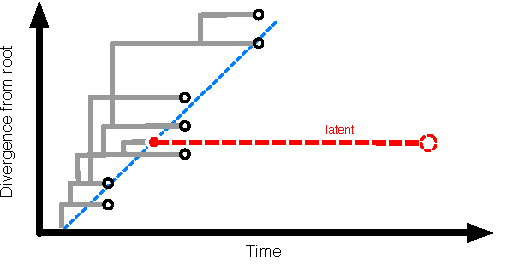
\includegraphics[width=10cm]{latency-scheme}
	\caption{%
	\csentence{Reconstructing the time that a viral lineage entered a latent state from with-host sequence variation.}
	A dashed line illustrates the linear relationship between the divergence of lineages from the ancestral sequence at the root ($y$-axis) and passage of time since the root ($x$-axis).
	Grey lines represent the reconstructed phylogenetic relationships among these lineages.
	The lineages were sampled (open circles) at three points in time.
	%Above is a time calibrated phylogeny with three taxa, the dotted line in is an example of latency. 
	One of these lineages had become latent at an earlier point in time (red hexagon).
	This lineage subsequently underwent negligible molecular evolution until it was sampled as integrated viral DNA (dashed circle).
	If the relationship between sequence divergence and time is sufficiently linear, then the time between latency establishment and sampling, here represented by the thick red dashed line, can be inferred from its sequence.
	%Sequence A was archived at time $t$, and was collected at the same time as sequence B, at time $t^\prime$ (a drift of $t^\prime - t$ is expected).
	%If the molecular clock assumption holds true, the MRCA is known, and B and C are reliable time-points, then the date at $t$ can be inferred from from the expected amount of evolution for B from the root.
	}
	\label{fig:latenttree}
\end{figure}


\begin{figure}[h!]
	\centering{}
	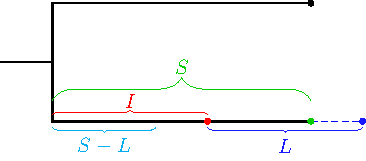
\includegraphics[width=10cm]{latency-model}
	\caption{%
	\csentence{Model simulating viral latency.}
	On a tip with branch length $S$, we randomly select a latency period, $L$ --- after which time the lineage would reactivate if it had not been sampled.
	Then we randomly select an integration period, $I$ --- the waiting period before integration --- between the interval $S-L$ and $S$.
	Here, $S-L$ is the earliest that the sequence could be integrated and still be sampled before activation.
	In the illustration, the red dot represents when teethe integration event of the lineage, the green dot represents when the lineage is sampled, and the blue dot represents when the lineage would have been reactivated if it was not sampled.
	}
	\label{fig:latencymodel}
\end{figure}

\begin{figure}[h!]
	\centering
	\includegraphics[width=12cm]{{Figure.3}.pdf}
	\caption{%
	\csentence{Simulated data.}
	The dotted line is the linear regression.
	(\subref{fig:resultssimulated}) shows an example from the \emph{simulated (no latency)} data set and (\subref{fig:resultslatent}) shows an example from the \emph{simulated (latency)} data set.
	The solid red lines in (\subref{fig:resultslatent}) connect the sampled dates of a lineage to its integration date.
	}
%	Patient: HIV_12
	\label{fig:results1}
	\sublabel{fig:resultssimulated}
	\sublabel{fig:resultslatent}		
\end{figure}

\begin{figure}[h!]
	\centering
	\includegraphics[width=12cm]{{Figure.4}.pdf}
	\caption{%
	\csentence{Real data.}
	As Figure \ref{fig:results1}, except for the real data.
	In (\subref{fig:resultslanl}), a putative latent lineage is circled in blue.
	A dashed blue line is drawn between the sampled sequence and its predicted integration time; this line represents the estimated period that the lineage was latent before being sampled.
	}
	\label{fig:results2}
	\sublabel{fig:resultsancre}
	\sublabel{fig:resultslanl}
\end{figure}

\begin{figure}[h!]
	\centering
	\includegraphics[width=12cm]{{Figure.5}.pdf}
	\caption{%
	\csentence{The densities of the scaled difference of each patient in the real data sets.}
	The solid lines represent the total density in the \emph{simulated (no latency)} data set for (\subref{fig:densityancre}) and \emph{simulated (latency)} data set for (\subref{fig:densitylanl}).
	}
	\label{fig:density}
	\sublabel{fig:densityancre}
	\sublabel{fig:densitylanl}
\end{figure}

\begin{figure}[h!]
	\centering
	\includegraphics[width=10cm]{patient\_16617}
	\caption{%
	\csentence{Patient 16617 from the \emph{mixed} data set.}
	Same as Figure \ref{fig:resultslanl} for Patient 16617 from the \emph{mixed} data set.
	The time between the green bars represents when the patient underwent therapy.
	The sequences circled in blue are likely to have latent lineages.
	}
	\label{fig:treatment}
\end{figure}

\clearpage{}

\section*{Additional file legends}
sm.pdf {\bf Additional file 1: Supplementary Materials, Figures, and Tables}. Results with outgroup rooting.

%%%%%%%%%%%%%%%  TABLES  %%%%%%%%%%%%%%%

%\section * {Tables}

%fs1.pdf {\bf Additional file 2: Figure S1}. Plot from the \emph{simulated (extreme latency)} data set of the evolutionary distance vs time.

%fs2.pdf {\bf Additional file 3: Figure S2}. Real data with outgroup rooting

%fs3.pdf {\bf Additional file 4: Figure S3}. Patient 16617 with outgroup rooting.

%ts1.pdf {\bf Additional file 5: Table S1}. Details of the linear model Details of the linear models applied to the real data sets using outgroup rooting.

\end{backmatter}

\end{document}
